% This file was created by tikzplotlib v0.9.8.
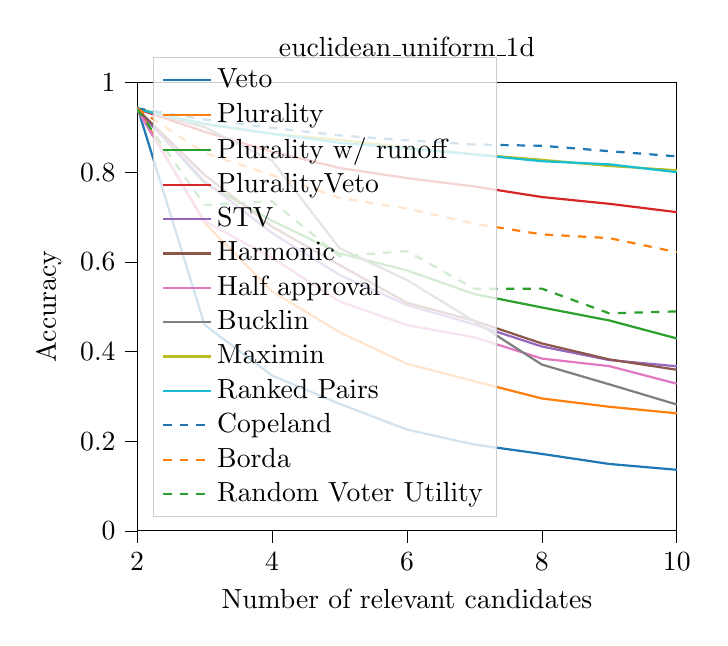
\begin{tikzpicture}

\definecolor{color0}{rgb}{0.12156862745098,0.466666666666667,0.705882352941177}
\definecolor{color1}{rgb}{1,0.498039215686275,0.0549019607843137}
\definecolor{color2}{rgb}{0.172549019607843,0.627450980392157,0.172549019607843}
\definecolor{color3}{rgb}{0.83921568627451,0.152941176470588,0.156862745098039}
\definecolor{color4}{rgb}{0.580392156862745,0.403921568627451,0.741176470588235}
\definecolor{color5}{rgb}{0.549019607843137,0.337254901960784,0.294117647058824}
\definecolor{color6}{rgb}{0.890196078431372,0.466666666666667,0.76078431372549}
\definecolor{color7}{rgb}{0.737254901960784,0.741176470588235,0.133333333333333}
\definecolor{color8}{rgb}{0.0901960784313725,0.745098039215686,0.811764705882353}

\begin{axis}[
legend cell align={left},
legend style={
  fill opacity=0.8,
  draw opacity=1,
  text opacity=1,
  at={(0.03,0.03)},
  anchor=south west,
  draw=white!80!black
},
tick align=outside,
tick pos=left,
title={euclidean\_uniform\_1d},
x grid style={white!69.0196078431373!black},
xlabel={Number of relevant candidates},
xmin=2, xmax=10,
xtick style={color=black},
y grid style={white!69.0196078431373!black},
ylabel={Accuracy},
ymin=0, ymax=1,
ytick style={color=black}
]
\addplot [thick, color0]
table {%
2 0.9464
3 0.4592
4 0.3464
5 0.2833
6 0.2258
7 0.1924
8 0.1715
9 0.1491
10 0.1361
};
\addlegendentry{Veto}
\addplot [thick, color1]
table {%
2 0.9448
3 0.6868
4 0.534
5 0.443
6 0.3725
7 0.3337
8 0.2952
9 0.2767
10 0.2621
};
\addlegendentry{Plurality}
\addplot [thick, color2]
table {%
2 0.942
3 0.7755
4 0.6918
5 0.6189
6 0.5809
7 0.528
8 0.4982
9 0.4692
10 0.4291
};
\addlegendentry{Plurality w/ runoff}
\addplot [thick, color3]
table {%
2 0.9412
3 0.89
4 0.8456
5 0.8095
6 0.7867
7 0.7681
8 0.7445
9 0.7294
10 0.7108
};
\addlegendentry{PluralityVeto}
\addplot [thick, color4]
table {%
2 0.9393
3 0.7801
4 0.6643
5 0.5708
6 0.5035
7 0.4603
8 0.4111
9 0.3809
10 0.367
};
\addlegendentry{STV}
\addplot [thick, color5]
table {%
2 0.9405
3 0.7937
4 0.6784
5 0.5931
6 0.5087
7 0.4685
8 0.4179
9 0.3823
10 0.3592
};
\addlegendentry{Harmonic}
\addplot [thick, color6]
table {%
2 0.939
3 0.6907
4 0.6091
5 0.5118
6 0.4587
7 0.4317
8 0.3842
9 0.3673
10 0.3281
};
\addlegendentry{Half approval}
\addplot [thick, white!49.8039215686275!black]
table {%
2 0.9414
3 0.9
4 0.8258
5 0.6304
6 0.5594
7 0.4674
8 0.3708
9 0.3267
10 0.2817
};
\addlegendentry{Bucklin}
\addplot [thick, color7]
table {%
2 0.9417
3 0.9067
4 0.8857
5 0.8719
6 0.8546
7 0.8398
8 0.8276
9 0.8138
10 0.8043
};
\addlegendentry{Maximin}
\addplot [thick, color8]
table {%
2 0.9406
3 0.908
4 0.8858
5 0.8654
6 0.853
7 0.8394
8 0.8244
9 0.8174
10 0.8
};
\addlegendentry{Ranked Pairs}
\addplot [thick, color0, dashed]
table {%
2 0.9423
3 0.9174
4 0.8988
5 0.882
6 0.871
7 0.8615
8 0.8589
9 0.8468
10 0.8352
};
\addlegendentry{Copeland}
\addplot [thick, color1, dashed]
table {%
2 0.9421
3 0.8426
4 0.7936
5 0.7427
6 0.7187
7 0.685
8 0.6612
9 0.6529
10 0.6216
};
\addlegendentry{Borda}
\addplot [thick, color2, dashed]
table {%
2 0.9404
3 0.7267
4 0.7351
5 0.6124
6 0.6239
7 0.5398
8 0.5402
9 0.4851
10 0.4894
};
\addlegendentry{Random Voter Utility}
\end{axis}

\end{tikzpicture}
